\chapter{Analýza}

V této kapitole je provedena analýza požadavků a je navržena architektura
výsledné aplikace.



\section{Požadavky}

\subsection{Nefunkční požadavky}

Výsledný navrhovaný nástroj musí splňovat následující podmínky

\subsubsection*{Implementace v jazyce Java}

Vzhledem k tomu, že důvodem ke vzniku práce bylo dodání licencovacího mechanismu
do existujících aplikací napsaných v jazyce Java, jedním z hlavních požadavků
je celý navržený systém implementovat v Javě. Ačkoliv Java umožňuje využívat
knihovny napsané například v C/C++ pomocí JNI\cite{jni} nebo JNA\cite{jna}, je
použití nativních knihoven mnohem snadnější.


\subsubsection*{Podpora pro aplikace napsané na platformě Eclipse RCP}

Důvodem tohoto požadavku je fakt, že existující aplikace jsou napsány právě na
platformě Eclipse RCP\cite{eclipse-rcp}. Pro snadnější integraci by měla být
klientská část navrhovaného systému distribuovaná v podobě pluginu.

Důsledkem tohoto požadavku je kromě podoby výsledné distribuce klientské části
také omezení týkající se knihoven třetích stran. Využívany by měli být především
takové knihovny, které jsou obvykle obsaženy ve většině distribucí aplikací
napsaných na platformě Eclipse RCP. Například v případě použití GUI by měla být
použita knihovna SWT\cite{swt}.

\subsubsection*{Funkčnost na operačních systémech Windows a Linux}

Tento požadavek opět souvisí s tím, že existující aplikace podporují právě tyto
operační systémy. Navíc jsou systémy Windows a Linux nejsnáze dostupné pro
testovací účely. 

Ačkoliv je Java multiplatformní jazyk, možnosti týkající se zístkávání informací
specifických pro konkrétní operační systém jsou značně omezené. Pokud chceme
vázat licenci na konkrétní hardware, je zapotřebí mnohem těsnější vazby s
operačním systémem, než jakou Java umožňuje. Z tohoto důvodu bude nutné část
funkcionality přizpůsobit konkrétnímu operačnímu systému a tuto část
implementovat pro všechny podporované platformy. Jako cílové byly zvoleny
operační systémy Windows a Linux, mělo by ale být možné v případě potřeby snadno
rozšířit podporu i pro další operační systémy.


\subsubsection*{Snadná integrovatelnost do již existujících aplikací}
 
K rozhodnutí o přidání funkčnosti pro licencování do aplikace může dojít až v
pozdější fázi vývoje, případně může být požadavek licencování přidat do již
hotového produktu. Z tohoto důvodu by měla být integrace co nejjednodušší.
Modulární architektura platformy Eclipse RCP toto v případě integrace do
desktopové aplikace usnadní. Stejný požadavek ale můžemem mít také na serverové
straně. Pokud již máme existující databázi uživatelů, mohli bychom ji chtít
využít pro vystavení licencí.
  
\subsubsection*{Centrální správa licencí}

Aby bylo možné mít přehled o všech vydaných licencích, je nutné licence
spravovat centrálně.

\subsubsection*{Webové GUI pro snadnějš správu licencí}

Protože o vydávání licencí se běžně stará obchodní oddělení, je potřeba
vytvořit grafické uživatelské rozhraní, které umožní uživatelům spravovat vydané
licence. Z hlediska snadnosti použití a platformní nezávislosti se jako
nejvhodnější jeví webové rozhraní.


\subsection{Funkční požadavky}

\subsubsection*{Vlastnosti licence}

Licence vydávané a ověřované implementovaným licenčním nástrojem musí mít
následující vlastnosti.

\begin{itemize}
  \item Časové omezení – počátek nebo konec platnosti licence je možné časově
  omezit
  \item Vazba na hardware – platnost licence je možné vázat na konkrétní
  hardware
  \item Licencované vlastnosti - do vystavené licence je možné zanést
  informace o povolených vlastnostech licencovaného produktu. Licencované
  vlastnosti je možné přidávat a odebírat
\end{itemize}

\subsubsection*{Vlastnosti klientské části}

Tyto vlastnosti bude mít klientská část licenčního mechanismu, která se bude
zabudovávat do aplikace.

\begin{itemize}
  \item Online kontrola platnosti – platnost licence bude je ověřit proti
  licenčnímu serveru.
  \item Offline kontrola platnosti – platnost údajů uvedených v licenci je
  možné ověřit bez nutnosti připojení k centrálnímu serveru. Jedná se především
  o kontrolu dat počátku a konce platnosti a kontroly vazby na hardware.
\end{itemize}

\subsubsection*{Vlastnosti serverové části}

\begin{itemize}
  \item Zobrazení přehledu vystavených licencí
  \item Vytvoření nové licence
  \item Zneplatnění licence
  \item Ověření platnosti vydané licence
\end{itemize}

\section{Architektura}

Jako nejvhodnější architektura pro navrhovaný produkt je typ klient-server.
Rozvržení jednotlivých komponent je zobrazeno v diagramu na obrázku
\ref{fig:deployment}.

\begin{figure}[tbh]
\begin{center}
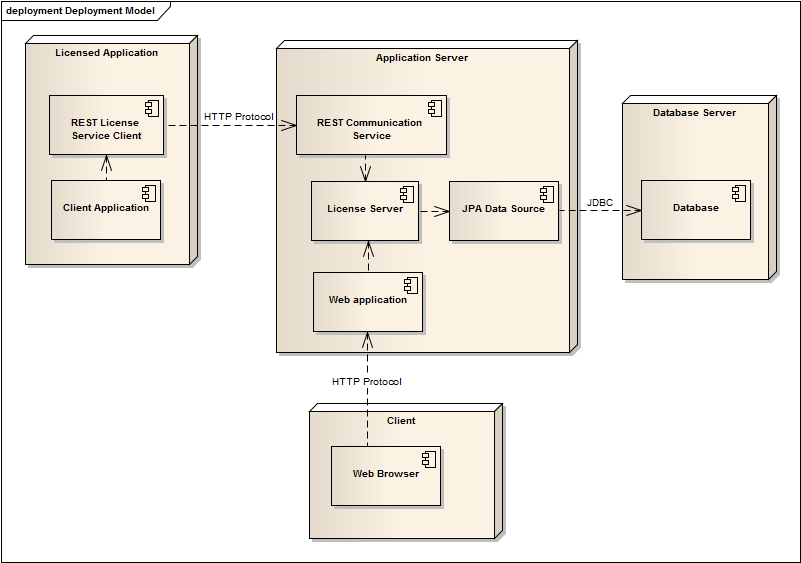
\includegraphics[width=11cm]{figures/deployment.png}
\caption{Diagram nasazení jednotlivých komponent}
\label{fig:deployment} 
\end{center}
\end{figure}

\subsection{Serverová část}

Účelem serverové části je poskytovat informace o vydaných licencích a ověřovat
jejich platnost. Serverová část může být integrována do existující serverové
aplikace, nebo nasazena jako samostatná aplikace. Komponenty serverové aplikace
jsou na obrázku \ref{fig:components-server}.


\begin{figure}[tbh]
\begin{center}
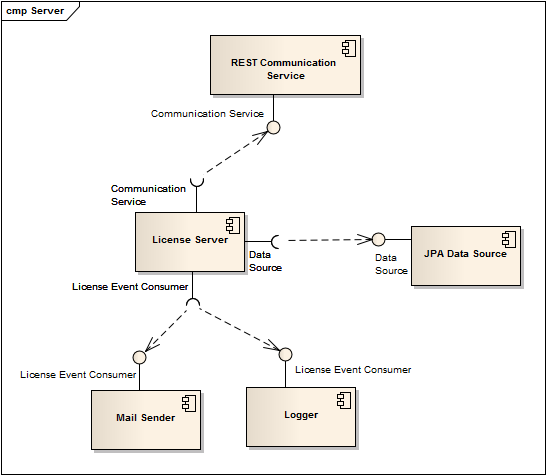
\includegraphics[width=11cm]{figures/components-server.png}
\caption{Diagram komponent serverové části}
\label{fig:components-server} 
\end{center}
\end{figure}

Pro zajištění rozšiřitelnosti, snadné integrace do existujících aplikací a dobré
testovatelnosti je část funkcionality serverové části rozdělena do několika
komponent s definovaným rozhraním.

\subsubsection*{License Server}

License Server je hlavní část serverové aplikace obsahující logiku spojenou s
ověřováním licencí. Jejím úkolem je odpovídat na požadavky od klientských aplikací na
ověření platnosti licence uložené v databázi. Jendotlivé části zajišťující
komunikaci s klienty a databází jsou dekomponovány do samostatných částí a
komunikace s nimi probíhá pomocí pevně daného rozhraní. To umožňuje udržet
komponentu nezávislou na použitém komunikačním protokolu a databázové vrstvě.

\subsubsection*{Communication Service}
\label{subsec:comm-service}

Communication Service je komponenta odpovědná za komunikaci s klientskými
aplikacemi. Jejím vyčleněním do samostatné části je dosaženo odstranění
závislosti na použitém protokolu pro komunikaci s klientskými aplikacemi.
Komponenta Communication Service překládá požadavky na ověření platnosti licence
z podoby specifické pro použitý komunikační protokol (\gls{XML}, \gls{JSON},
Serialozované objekty, \ldots) do univerzální podoby akceptované částí License Server.

\subsubsection*{Data Source}

Komponenta Data Source slouží k načítání a ukládání informací o vydaných
licencích do persistentního úložiště. Poskytuje serverové aplikaci základní operace jako
nalezení licence podle identifikátoru a zaznamenání aktivace licence. Při
integraci serverové části do již existující aplikace je komponenta Data Source
použita pro napojení na existující datový model. V případě samostatného nasazení
může být komponenta naimplementována jako \gls{DAO}.

\subsubsection*{License Event Consumer}

Poslední z navržených komponent je komponenta s názvem License Event Consumer. 
Účelem této komponenty je umožnit snadnější rozšíření serverové aplikace o
dodatečnou funkcionalitu. Jendá se o aplikaci návrhového vzoru observer –
komponenta License Server umožní registrovat komponenty implementující rozhraní
License Event Consumer. Registrované komponenty budou notifikovány o událostech
v serverové aplikaci, například při povolení nebo zamítnutí ověření licence.
Tímto způsobbem je možné doplnit aplikaci o další funkcionalitu, například
logování událostí nebo zasílání notifikací pomocí emailu.


\subsection{Klientská část}

Klientoskou částí se rozumí část vyvíjeného nástroje, která se zabuduje do
licencované aplikace. Účelem této části je poskytnout licencované aplikaci
programové rozhraní pro vyžádání a ověření licence. Rozdělení klientské části na
jednotlivé komponenty je zobrazena na obrázku \ref{fig:components-client}.

\begin{figure}[tbh]
\begin{center}
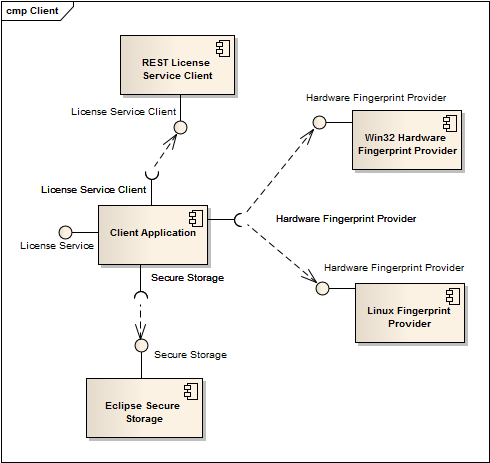
\includegraphics[width=11cm]{figures/components-client.png}
\caption{Diagram komponent klientské části}
\label{fig:components-client} 
\end{center}
\end{figure}

Klientská část je podobně jako serverová část rozdělená do na jendotlivé
komponenty. Jedná se ale především o logické dělení – při integraci do cílové
aplikace mohou být jednotlivé komponenty mnohem těsněji provázány za účelem
znesnadnění odstranění jednotlivých částí.

\subsubsection*{Client Application}

Client Application je hlavní komponenta klientské aplikace obsahující všechnu
potřebnou logiku. Účelem této komponenty je poskytovat aplikaci informace o
aktuální licenci a případně umožnit aplikaci si vyžádat aktivaci nové licence.
%TODO

\subsubsection*{License Service Client}
\label{subsec:license-service-client}

Komponenta License Service Client slouží ke komunikaci se serverovou aplikací.
Jedná se o protějšek serverové komponenty Communication Service. Vyčleněním
komunikace se serverem do samostatné komponenty získáme možnost změny
komunikačního protokolu bez nutnosti zásahu do ostatních částí klientské
aplikace.

\subsubsection*{Hardware Fingerprint Provider}

Účelem komponenty Hardware Fingerprint Provider je poskytnout klientské části
přístup k informacím o hardware počítače, na kterém je licencovaná aplikace
nainstalována. Informace o hardware počítače jsou použity pro vytvoření
unikátního otisku hardware. Protože že vyvýjený licencovací nástroj
musí být funkční na operačních systémech Windows a Linux, je nutné tuto
funkcionalitu vyčelnit do samostatné komponenty. 

\subsubsection*{Secure Storage}

Jedním z požadavků na klientskou část je možnost ověřit platnost licence bez
aktivního připojení na internet. Z toho důvodu je nutné mít informace o
aktivované licenci uložené, aby je bylo možné při opětovném spuštění aplikace
načíst a ověřit. Za tímto účelem je navržena komponenta Secure Storage. Cílem
této komponenty je poskytnout klientské aplikaci persistentní úložiště pro
informace o licenci. Persistentní podoba uložené licence musí být chráněna proti
modifikaci z venčí.

\subsubsection*{License Service}
 
Rozhraní License Service je jediná část licencovacího nástroje viditelná z
klientské aplikace. Umožňuje klientské aplikaci provést ověření aktuální licence
a v případě potřeby vyžádání nové licence.

\section{Doménový model}



\section{Komunikace}

V návrhu architektury licencovacího nástroje je v
sekci~\ref{subsec:comm-service} navržena serverová komponenta pro komunikaci s
klientskými aplikacemi, v sekci~\ref{subsec:license-service-client} je popsán
její protějšek umístěný v klientské aplikaci. Komponenty umožňují použití
libovolného komunikačního protokolu mezi klientskou a serverovou částí, v
navrhovaném licencovacím nástroji bude tato část implementována v podobě RESTful
webové služby.

Architektura \gls{REST} byla vybrána z následujících důvodů:
\begin{itemize}
  \item Komunikace probíhá pomocí protokolu \gls{HTTP}. To je výhodné například
  při použití v podnikovém prostředí, kde kromě \gls{HTTP} protokolu bývají
  ostatní komunikační protokoly omezené nebo zakázané.
  \item Jazyk Java obsahuje nativní podporu pro komunikaci pomocí protokolu
  \gls{HTTP}, na klientské straně nejsou potřeba žádné další knihovny.
  \item Protokol \gls{HTTP} je bezestavový, což zjednodušuje implementaci.
  \item Protokol \gls{HTTP} není vázán pouze na jazyk Java, serverovou část je
  možné volat i z klientů napsaných v jiných jazycích.
\end{itemize}

\subsection{REST}

\gls{REST} je koncept pro návrh distribuované architektury, u které je
komunikace realizována pomocí protokolu \gls{HTTP}. \gls{REST} webové služby
jsou orientovány na práci s datovými zdroji. Každý zdroj má svůj unikátní
identifikátor (\gls{URN}), pomocí něhož se s daným zdrojem manipuluje. Rozlišují
se čtyři základní operace:

\begin{itemize}
  \item Create - vytvoření zdroje, na úrovni protokolu \gls{HTTP} se pro tuto
  operaci používá metoda PUT.
  \item Read - čtení informací z datového zdroje, pro tuto operaci se používá
  metoda GET.
  \item Update - upravení informací zdroje, nejčastěji realizováno metodou POST
  \item Delete - smazání datového zdroje, pro tuto operaci se používá metoda
  DELETE.
\end{itemize}

Výsledek provedené operace je klientovi sdělen pomocí návratového kódu
\gls{HTTP}. Nejčastěji se používají následující návratové kódy:

\begin{itemize}
  \item 200 OK - Kód označuje, že požadavek byl proveden úspěšně.
  \item 400 Bad Request - Kód vrácen v případě, že požadavek od klienta je
  špatně zfromulován, nebo obsahuje neplatné údaje.
  \item 404 Not Found - Kód označující, že požadovaný zdoj nebyl nalezen.
  \item 500 Internal Server Error - Kód vrácen v případě, že při zpracování
  došlo k chybě naserveru.
\end{itemize}

Kompletní přehled stavových kódu \gls{HTTP} lze nalézt ve specifikaci
\cite{rfc-http}.

Pokud chce klient například získat informace o licenci 12345, komunikace bude
vypadat následovně:

\begin{enumerate}
  \item Klient pošle \gls{HTTP} požadadavek na adresu
  http://server/licence/12345
  \item Server přijme požadavek a vyhledá licenci s identifikátorem 12345.
  \item Server odešle klientovi odpověď s návratovým kódem 200. Informace o
  licenci budou obsaženy v těle odpovědi ve formátu \gls{XML}.
\end{enumerate}

\subsection{Serverové rozhranní}

Serverová část poskytne klientům pomocí \gls{REST} webové služby metody pro
práci s licencemi.

\subsubsection*{Zažádání o aktivaci licence}

Serverová část umožní klientským aplikacím zažádat o aktivaci licence. Aktivace
se provede pomocí \gls{HTTP} dotazu typu POST na \gls{URL} /activations. V
požadavku klient uvede:

\begin{itemize}
  \item Identifikátor licence, kterou chce klientská aplikace aktivovat.
  \item Hardwarový otisk počítače, ze kterého je prováděna aktivace.
\end{itemize}

Server zpracuje požadavek, možné odpovědi jsou uvedeny v tabulce \ref{tab:license-request-responses} 

\begin{table}\centering
	\caption[Results]{Seznam možných odpovědí
	serveru na požadavek na akitvaci licence}\label{tab:license-request-responses}
	\begin{tabular}{|p{1cm}|p{3cm}|p{4cm}|p{3cm}|}\hline 
	Kód		&  Popis	& Obsah těla odpovědi & Položky v hlavičce odpovědi
	\tabularnewline \hline \hline 
	201		& Licence úspěšně vytvořena	& Textová reprezentace nově vytvořené aktivace
	& parametr Location s adresou nově vytvořené aktivace
	\tabularnewline \hline
	TODO	& Požadovaná licence nenalezena & Informace o typu chyby & -
	\tabularnewline \hline
	403		& Platnost licence vypršela & Informace o typu chyby a platnosti licence &
	-
	\tabularnewline \hline
	403		& Licence zneplatněna	& Informace o typu chyby & -
	\tabularnewline \hline
	403 	& Vyčerpán počet aktivací & Informace o typu chyby, maximální počet
	aktivací & -
	 \tabularnewline \hline
	\end{tabular}
\end{table}

\subsubsection*{Získání informace o aktivaci licence}

Serverová část umožní klientským aplikacím získat informace o aktivaci licence
provedením \gls{HTTP} dotazu typu GET bez těla na adresu
/activations/\{identifikátor~aktivace\}.

Možné odpovědi serveru jsou v tabulce \ref{tab:activation-request-responses}


\begin{table}\centering
	\caption[Results]{Seznam možných odpovědí
	serveru na požadavek na informace o akitvaci
	licence}\label{tab:activation-request-responses} \begin{tabular}{|p{1cm}|p{3cm}|p{4cm}|p{3cm}|}\hline 
	Kód		&  Popis	& Obsah těla odpovědi & Položky v hlavičce odpovědi
	\tabularnewline \hline \hline 
	200		& Aktivace nalzena	& Textová reprezentace údajů o aktuïvaci licence
	& -
	\tabularnewline \hline
	404	& Požadovaná aktivace licence nenalezena & - & -
	\tabularnewline \hline
	\end{tabular}
\end{table}

\subsection{Zabezpečení komunikace}

Informace jsou u \gls{HTTP} protokolu přenášeny v čitelné textové podobě. Tím
vznikají následující rizika:

\begin{itemize}
  \item Útočník může odposlechnout přenášená data. Při komunikaci s licenčním
  serverem se nepřenášejí žádné důvěrné informace (například údaje o klientovi),
  útočník ale může získat identifikátor licence a pomocí něj si aktivovat
  vlastní kopii licencovaného software.
  \item Útočník může pozměnit obsah zprávy, případně komunikaci se serverem
  podvrhnout. Tím by bylo možné si například změnit typ licence nebo do
  licence přidat vlastnosti, ačkoliv je uživatel nemá v licenci zahrnuty.
\end{itemize}

Pokud zamezit odposlechu komunikace, klientská aplikace umožní použít ke
komunikaci namísto nešiforvaného protokolu \gls{HTTP} bezpečnější šifrovanou
verzi \gls{HTTPS}. Nevýhodou tohoto řešní je nutnost mít v klientské aplikaci i
na serveru nainstalovaný důvěryhodný certifikát, pomocí něhož se bude komunikace
šifrovat.

Možností, jak zamezit modifikaci požadavku mezi klientskou a serverovou
aplikací, je použití digitálního podpisu. Do hlavičky každého požadavku se
připojí kontrolní součet těla požadavku zašifrovaný klíčem klienta nebo
serveru. Tím bude možné zkontrolovat, že zpráva byla přenesená bez modifikace.
Zároveň se tím potvrdí identita odesílatele zprávy.


